\chapter{Specifikacija programske potpore}
		
	\section{Funkcionalni zahtjevi}

			%\textbf{\textit{dio 1. revizije}}\\
					
			\noindent \textbf{Dionici:}
			
			\begin{packed_enum}
				
				\item Dionik 1
				\item Dionik 2				
				\item ...
				
			\end{packed_enum}
			
			\noindent \textbf{Aktori i njihovi funkcionalni zahtjevi:}
			
			
			\begin{packed_enum}
				\item  \underbar{Aktor 1 (inicijator) može:}
				
				\begin{packed_enum}
					
					\item funkcionalnost 1
					\item funkcionalnost 2
					\begin{packed_enum}
						
						\item  podfunkcionalnost 1 
						\item  podfunkcionalnost 2
				
					\end{packed_enum}
					\item  funkcionalnost 3
					
				\end{packed_enum}
			
				\item  \underbar{Aktor 2 (sudionik) može:}
				
				\begin{packed_enum}
					
					\item funkcionalnost 1
					\item funkcionalnost 2
					
				\end{packed_enum}
			\end{packed_enum}
			
			\eject 
			
			
				
			\subsection{Obrasci uporabe}
				
				%\textbf{\textit{dio 1. revizije}}
				
				\subsubsection{Opis obrazaca uporabe}			

					\noindent \underbar{\textbf{UC1 - Registracija}}
					\begin{packed_item}
	
						\item \textbf{Glavni sudionik: }Javni korisnik
						\item  \textbf{Cilj:} Stvaranje računa za pristup stranici
						\item  \textbf{Sudionici:} Baza podataka
						\item  \textbf{Preduvjet:} -
						\item  \textbf{Opis osnovnog tijeka:}
						
						\item[] \begin{packed_enum}
							\item Korisnik unosi potrebne korisničke podatke
							\item Korisnik na upisanu mail adresu dobiva potvrdu o uspješnoj registraciji
						\end{packed_enum}
						
						\item  \textbf{Opis mogućih odstupanja:}

						\item[] \begin{packed_item}
						%\item[] 
							\item[2.a] Unos već zauzete ili krive email adrese, unos podataka u neispravnom formatu
							\item[] \begin{packed_enum}
								
								\item Korisnik dobiva obavijest o pogrešci i ponovno se nalazi na stranici za registraciju
								\item Korisnik ispravlja neispravne podatke i završava unos ili odustaje od registracije
								
							\end{packed_enum}					
						\end{packed_item}
					\end{packed_item}

					\noindent \underbar{\textbf{UC2 - Prijava u sustav}}
					\begin{packed_item}
	
						\item \textbf{Glavni sudionik: }Registrirani korisnik
						\item  \textbf{Cilj:} Pristup početnoj stranici kao prijavljeni korisnik
						\item  \textbf{Sudionici:} Baza podataka
						\item  \textbf{Preduvjet:} -
						\item  \textbf{Opis osnovnog tijeka:}
						
						\item[] \begin{packed_enum}
							\item Korisnik unosi email adresu i lozinku
							\item Korisnik pri uspješnom unosu podataka biva preusmjeren na početnu stranicu
						\end{packed_enum}
						
						\item  \textbf{Opis mogućih odstupanja:}

						\item[] \begin{packed_item}
						%\item[] 
							\item[1.a] Unos neispravne email adrese ili zaporke
							\item[] \begin{packed_enum}
								
								\item Korisnik dobiva obavijest o unosu neispravnih podataka
								\item Korisnik ispravlja neispravne podatke i završava unos ili odustaje od prijave
								
							\end{packed_enum}					
						\end{packed_item}
					\end{packed_item}

					\eject

					\noindent \underbar{\textbf{UC3 - Pregled osobnih podataka}}
					\begin{packed_item}
	
						\item \textbf{Glavni sudionik: }Prijavljeni korisnik
						\item  \textbf{Cilj:} Pregled podataka o korisniku
						\item  \textbf{Sudionici:} Baza podataka
						\item  \textbf{Preduvjet:} Korisnik se uspješno prijavio u sustav
						\item  \textbf{Opis osnovnog tijeka:}
						
						\item[] \begin{packed_enum}
							\item Korisnik odabire opciju za prikaz osobnih podataka
							\item Korisnik na stranici vidi prikaz svojih osobnih podataka
						\end{packed_enum}

						\item  \textbf{Opis mogućih odstupanja:}

						\item[] \begin{packed_item}
						%\item[] 
							\item[2.a] Baza ne uspije poslati podatke o korisniku
							\item[] \begin{packed_enum}
								
								\item Korisnik dobiva obavijest o neuspješnom dohvatu podataka
								\item Korisnik osvježava stranicu ili odustaje od pregleda osobnih podataka
							
							\end{packed_enum}	
						\end{packed_item}
						
					\end{packed_item}

					\noindent \underbar{\textbf{UC4 - Uređivanje osobnih podataka}}
					\begin{packed_item}
	
						\item \textbf{Glavni sudionik: }Prijavljeni korisnik
						\item  \textbf{Cilj:} Promjena osobnih podataka korisnika
						\item  \textbf{Sudionici:} Baza podataka
						\item  \textbf{Preduvjet:} Korisnik se uspješno prijavio u sustav
						\item  \textbf{Opis osnovnog tijeka:}
						
						\item[] \begin{packed_enum}
							\item Korisnik odabire opciju za uređivanje osobnih podataka
							\item Korisnik na stranici mijenja unesene osobne podatke
							\item Korisnik potvrđuje promjene
							\item Ažuriranje baze podataka pri potvrđenoj promjeni
						\end{packed_enum}

						\item  \textbf{Opis mogućih odstupanja:}

						\item[] \begin{packed_item}
						%\item[] 
							\item[2.a] Korisnik promijeni osobne podatke, ali ne potvrdi promjene
							\item[] \begin{packed_enum}
								
								\item Korisnik dobiva obavijest o nepotvrđenom unosu podataka prije \newline odlaska sa stranice
								\item Korisnik potvrđuje podatke ili odustaje od promjene podataka
							
							\end{packed_enum}	
							\item[4.a] Baza se ne uspije ažurirati
							\item[] \begin{packed_enum}
							
								\item Korisnik dobiva obavijest o neuspješnom ažuriranju baze podataka
								\item Korisnik ponovno potvrđuje podatke ili odustaje od promjene \newline podataka
							\end{packed_enum}
						\end{packed_item}
						
					\end{packed_item}

					\eject

					\noindent \underbar{\textbf{UC5 - Uređivanje podataka o djeci}}
					\begin{packed_item}
	
						\item \textbf{Glavni sudionik: }Prijavljeni korisnik
						\item  \textbf{Cilj:} Promjena podataka o djeci korisnika
						\item  \textbf{Sudionici:} Baza podataka
						\item  \textbf{Preduvjet:} Korisnik se uspješno prijavio u sustav
						\item  \textbf{Opis osnovnog tijeka:}
						
						\item[] \begin{packed_enum}
							\item Korisnik odabire opciju za uređivanje podataka o djeci
							\item Korisnik na stranici mijenja ili dodaje podatke o djeci
							\item Korisnik potvrđuje promjene
							\item Ažuriranje baze podataka pri potvrđenoj promjeni
						\end{packed_enum}

						\item  \textbf{Opis mogućih odstupanja:}

						\item[] \begin{packed_item}
						%\item[] 
							\item[2.a] Korisnik promijeni podatke o djeci, ali ne potvrdi promjene
							\item[] \begin{packed_enum}
								
								\item Korisnik dobiva obavijest o nepotvrđenom unosu podataka prije \newline odlaska sa stranice
								\item Korisnik potvrđuje podatke ili odustaje od promjene podataka
							
							\end{packed_enum}	
							\item[4.a] Baza se ne uspije ažurirati
							\item[] \begin{packed_enum}
							
								\item Korisnik dobiva obavijest o neuspješnom ažuriranju baze podataka
								\item Korisnik ponovno potvrđuje podatke ili odustaje od promjene \newline podataka
							\end{packed_enum}
						\end{packed_item}
						
					\end{packed_item}

					\noindent \underbar{\textbf{UC6 - Pregled oglasa}}
					\begin{packed_item}
	
						\item \textbf{Glavni sudionik: }Prijavljeni korisnik
						\item  \textbf{Cilj:} Pregled svih aktivnih oglasa
						\item  \textbf{Sudionici:} Baza podataka
						\item  \textbf{Preduvjet:} Korisnik se uspješno prijavio u sustav
						\item  \textbf{Opis osnovnog tijeka:}
						
						\item[] \begin{packed_enum}
							\item Korisnik odabire opciju za odlazak na početnu stranicu
							\item Na početnoj stranici su korisniku prikazani svi aktivni oglasi
						\end{packed_enum}

						\item  \textbf{Opis mogućih odstupanja:}

						\item[] \begin{packed_item}
						%\item[] 
							\item[2.a] Baza ne uspije poslati podatke o aktivnim oglasima
							\item[] \begin{packed_enum}
								
								\item Korisnik dobiva obavijest o neuspješnom dohvatu podataka
								\item Korisnik osvježava stranicu ili odustaje od pregleda aktivnih oglasa
							
							\end{packed_enum}	
						\end{packed_item}
						
					\end{packed_item}

					\eject
					\noindent \underbar{\textbf{UC7 - Filtriranje oglasa}}
					\begin{packed_item}
	
						\item \textbf{Glavni sudionik: }Prijavljeni korisnik
						\item  \textbf{Cilj:} Pregled oglasa iz određene kategorije/potkategorije
						\item  \textbf{Sudionici:} Baza podataka
						\item  \textbf{Preduvjet:} Korisnik se uspješno prijavio u sustav
						\item  \textbf{Opis osnovnog tijeka:}
						
						\item[] \begin{packed_enum}
							\item Korisnik odabire opciju za filtriranje oglasa po određenoj kategoriji ili potkategoriji
							\item Na početnoj stranici se korisniku prikažu oglasi koji zadovoljavaju zadane opcije filtriranja
						\end{packed_enum}

						\item  \textbf{Opis mogućih odstupanja:}

						\item[] \begin{packed_item}
						%\item[] 
							\item[2.a] Baza ne uspije poslati podatke o odgovarajućim oglasima
							\item[] \begin{packed_enum}
								
								\item Korisnik dobiva obavijest o neuspješnom dohvatu podataka
								\item Korisnik ponovno odabire opciju za filtriranje oglasa ili odustaje od filtriranja
							
							\end{packed_enum}	

							\item[2.b] Ne postoje oglasi koji odgovaraju zadanim opcijama filtriranja
							\item[] \begin{packed_enum}
								
								\item Korisnik dobiva obavijest o manjku odgovarajućih oglasa
								\item Korisnik mijenja opcije filtriranja ili odustaje od filtriranja oglasa
							
							\end{packed_enum}	

						\end{packed_item}
						
					\end{packed_item}

					\noindent \underbar{\textbf{UC8 - Pregled preporučenih oglasa}}
					\begin{packed_item}
	
						\item \textbf{Glavni sudionik: }Prijavljeni korisnik
						\item  \textbf{Cilj:} Pregled oglasa personaliziranih korisniku
						\item  \textbf{Sudionici:} Baza podataka
						\item  \textbf{Preduvjet:} Korisnik se uspješno prijavio u sustav
						\item  \textbf{Opis osnovnog tijeka:}
						
						\item[] \begin{packed_enum}
							\item Korisnik odabire opciju za prikaz preporučenih oglasa
							\item Na stranici se korisniku prikažu preporučeni oglasi
						\end{packed_enum}

						\item  \textbf{Opis mogućih odstupanja:}

						\item[] \begin{packed_item}
						%\item[] 
							\item[2.a] Baza ne uspije poslati podatke o odgovarajućim oglasima
							\item[] \begin{packed_enum}
								
								\item Korisnik dobiva obavijest o neuspješnom dohvatu podataka
								\item Korisnik ponovno odabire opciju za prikaz preporučenih oglasa ili odustaje od pregleda preporučenih oglasa
							
							\end{packed_enum}	
							\item[2.b] Ne postoje oglasi koji odgovaraju korisnikovim željama
							\item[] \begin{packed_enum}
								
								\item Korisnik dobiva obavijest o manjku odgovarajućih oglasa
								\item Korisnik odustaje od pregleda preporučenih oglasa
							
							\end{packed_enum}	
						\end{packed_item}
						
					\end{packed_item}

					\noindent \underbar{\textbf{UC9 - Poticanje donacija}}
					\begin{packed_item}
	
						\item \textbf{Glavni sudionik: }Prijavljeni korisnik
						\item  \textbf{Cilj:} Podsjećanje korisnika o mogućnosti doniranja primljenog predmeta
						\item  \textbf{Sudionici:} Baza podataka
						\item  \textbf{Preduvjet:} Korisnik se uspješno prijavio u sustav, korisnik ima primljene donacije
						\item  \textbf{Opis osnovnog tijeka:}
						
						\item[] \begin{packed_enum}
							\item Korisnik dobiva obavijest o mogućnosti doniranja primljenog predmeta
							\item Korisnik prihvaća mogućnost doniranja predmeta i biva preusmjeren na kreiranje oglasa
						\end{packed_enum}

						\item  \textbf{Opis mogućih odstupanja:}

						\item[] \begin{packed_item}
						%\item[] 
							\item[2.a] Korisnik odbija mogućnost doniranja predmeta
							\item[] \begin{packed_enum}
								
								\item Obavijest o mogućnosti doniranja se više ne prikazuje
							
							\end{packed_enum}	

						\end{packed_item}
						
					\end{packed_item}
					
				\subsubsection{Dijagram obrazaca uporabe}
					\begin{figure}[H]
						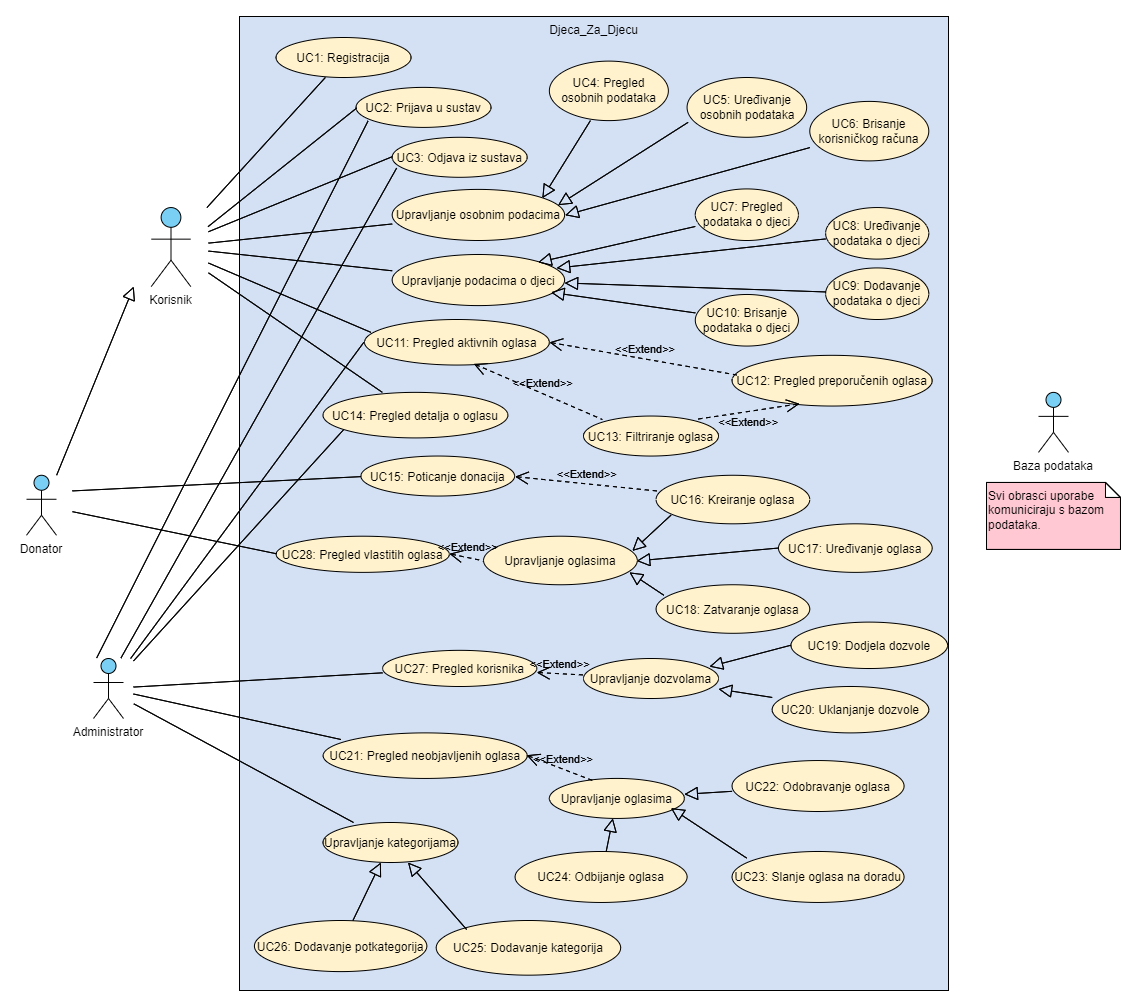
\includegraphics[width=\textwidth,height=0.7\textheight]{dijagrami/UCD - Djeca za djecu.png}
						\centering
						\caption{Dijagram obrazaca uporabe - aplikacija Djeca za djecu}
						\label{fig:useCaseDiagramMain}
					\end{figure}
					%\textit{Prikazati odnos aktora i obrazaca uporabe odgovarajućim UML dijagramom. Nije nužno nacrtati sve na jednom dijagramu. Modelirati po razinama apstrakcije i skupovima srodnih funkcionalnosti.}
				\eject
				
			\subsection{Sekvencijski dijagrami}
				
				%\textbf{\textit{dio 1. revizije}}\\
				
				\textit{Nacrtati sekvencijske dijagrame koji modeliraju najvažnije dijelove sustava (max. 4 dijagrama). Ukoliko postoji nedoumica oko odabira, razjasniti s asistentom. Uz svaki dijagram napisati detaljni opis dijagrama.}
				\eject
	
		\section{Ostali zahtjevi}
		
			%\textbf{\textit{dio 1. revizije}}\\
		 